\chapter{Informe final}

\section{Cálculo de parámetros experimentales - Rectificador trifásico media onda}

Para la obtención de parámetros eléctricos se tuvo como referencia implementación se hizo uso del esquema en la figura \ref{fig:circuito-rect-3p-half-wave} 

% TODO: \usepackage{graphicx} required
\begin{figure}[h]
	\centering
	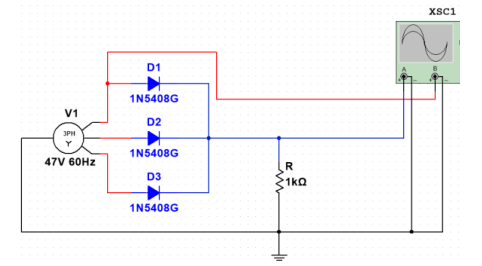
\includegraphics[width=0.7\linewidth]{media/circuito-rect-3p-half-wave}
	\caption{Circuito rectificador trifásico a media onda}
	\label{fig:circuito-rect-3p-half-wave}
\end{figure}

Y la cual se implemento de forma directa mediante el uso de componentes de protección como las borneras, cable vulcanizado además de los componentes necesarios para la rectificación como los diodos y resistencias, el circuito resultante se muestra en la figura \ref{fig:implementacion-rect-3p}

\begin{figure}[h]
	\centering
	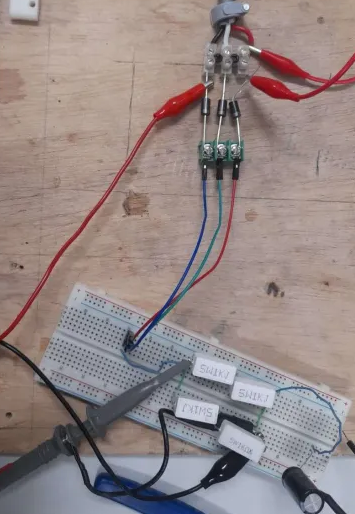
\includegraphics[width=0.7\linewidth]{media/implementacion-rect-3p}
	\caption{Implementación del circuito rectificador a media onda}
	\label{fig:implementacion-rect-3p}
\end{figure}

Por otro lado para la alimentación se tuvo en cuenta el módulo trifásico de potencia con una salida de 47V.

\begin{figure}[h]
	\centering
	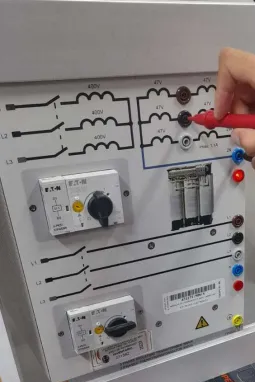
\includegraphics[width=0.7\linewidth]{media/entrada-trifasica}
	\caption{Fuente de alimentación trifásica}
	\label{fig:entrada-trifasica}
\end{figure}

Una vez configurados todos los parámetros requeridos para el funcionamiento se realizaron las conexiones adicionales para medir los parámetros eléctricos del circuito, esto como se puede apreciar en la figura \ref{fig:mediciones-salida} con una sonda en la entrada y salida del circuito. 

\begin{figure}[h]
	\centering
	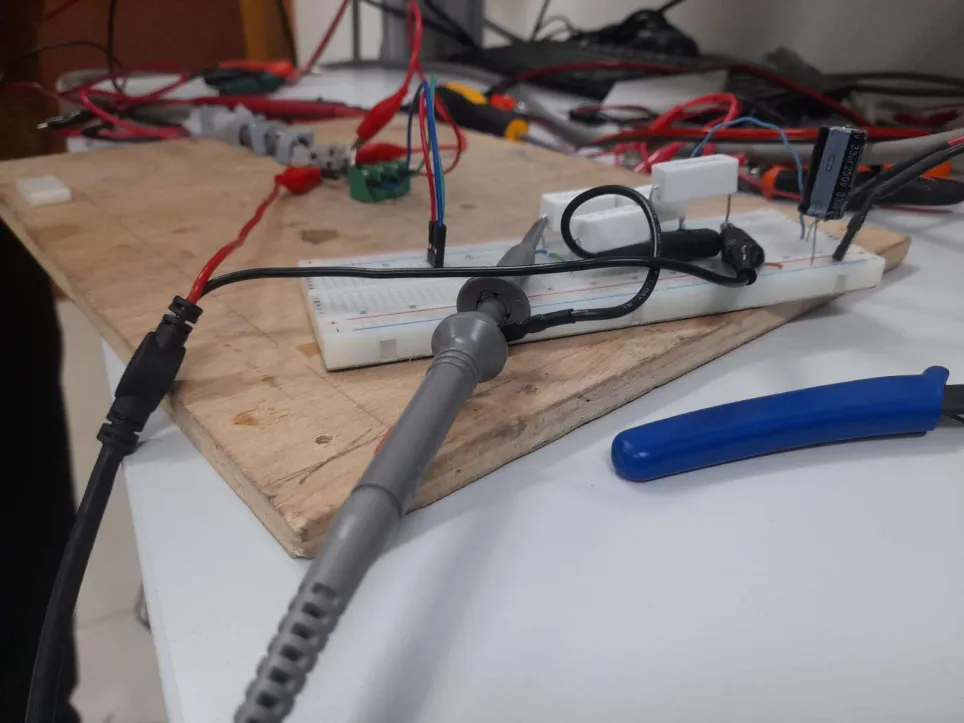
\includegraphics[width=0.7\linewidth]{media/mediciones-salida}
	\caption{Conexionado para obtener las parámetros electricos de salida}
	\label{fig:mediciones-salida}
\end{figure}

Obteniendo como resultado en la salida para una \textbf{carga R} la señal pulsante mostrada en la figura \ref{fig:senal-salida} 

\begin{figure}[h]
	\centering
	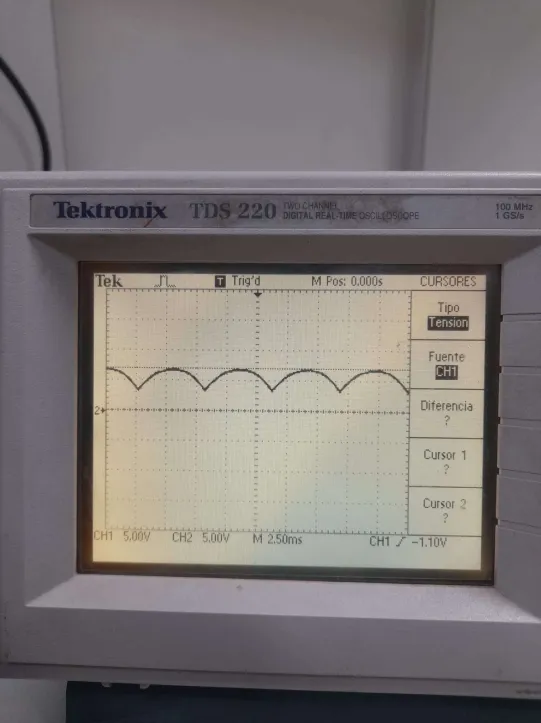
\includegraphics[width=0.7\linewidth]{media/senal-salida}
	\caption{Señal rectificada de salida - carga R}
	\label{fig:senal-salida}
\end{figure}

Para la cual se realizaron las mediciones para obtener los valores de rendimiento eléctricos 

\begin{multicols}{2}
	\noindent
	Voltaje pico, \( V_m \) = 67.8822v \\
	Voltaje medio, \( V_{\text{medio}} \) = 58.8v \\
	Voltaje eficaz, \( V_{\text{rms}} \) = 59.7 \\
	Corriente media, \( I_{\text{media}} \) = 0.05945 A \\
	Corriente eficaz, \( I_{\text{rms}} \) = 0.060364 A \\
	Rizado, \( r \) = 0.1756 \\
	Potencia en AC, \( P_{\text{ac}} \) = 3.603 \\
	Potencia en DC, \( P_{\text{dc}} \) = 3.4958\\
	Rendimiento, \( \eta \) = 0.9686\\
	Factor de forma, \( FF \) = 1.01530\\
	Factor de rizado, \( RF \) = 0.1756\\
	Factor de utilización (TUF) = 21.3737\\
	Factor de potencia, \( FP \) = 1.030846\\
	Voltaje pico inverso (PIV) = 117.5716 \\
	Corriente pico del diodo, \( I_p \) = 0.060364\\
	Frecuencia de salida, \( f_{\text{out}} \) = 180 \\
\end{multicols}

